\documentclass[12pt]{article}
\usepackage[a4paper, total={5.5in, 9in}]{geometry}
\usepackage{amsmath}
\usepackage{amsfonts}
\usepackage{graphicx}
\usepackage{pgfplots}
\pgfplotsset{compat=1.18}
\usepackage{enumitem}

\title{College Algebra Worksheet 3.7}
\author{PCL Learning Center}
\date{}

\begin{document}
\maketitle

\begin{center}
    \textit{note: No graphing calculators or electronic devices may be used on this worksheet.}    
\end{center}

\section*{Problem Set 1\\Difficulty level: Normal}
\subsection*{Problem 1}
Consider the function \(f\), which is a one-to-one function with values \(f(3)=2\) and \(f(-4)=8\).
    \begin{enumerate}[label=(\alph*)]
        \item \( f^{-1}(8) = 3 \)
        \item \( f^{-1}(2) = 8 \)
        \item \( f^{-1}(3) = -2 \)
        \item \( f^{-1}(2) = 3 \)
        \item \( f^{-1}(8) = -4 \)
        \item \( f^{-1}(-4) = -8 \)
    \end{enumerate}

\subsection*{Problem 2}
Use the following table of values for the one-to-one function \(g(x)\) to find \(g^{-1}(-3)\).
\[
\begin{array}{c|cccccc}
x & -6 & -3 & -1 & 5 & 8 & 11 \\
\hline
g(x) & -11 & -10 & -3 & 3 & 9 & 10 \\
\end{array}
\]

\subsection*{Problem 3}
You want to restrict the domain of the function shown in the graph below to make it one-to-one so that it will have an inverse. What are the largest domains in interval notation?\\
\textit{note: You want your answer to look like \([\hspace{0.2cm},\hspace{0.2cm}]\) or \([\hspace{0.2cm},\hspace{0.2cm}]\)}

\begin{center}
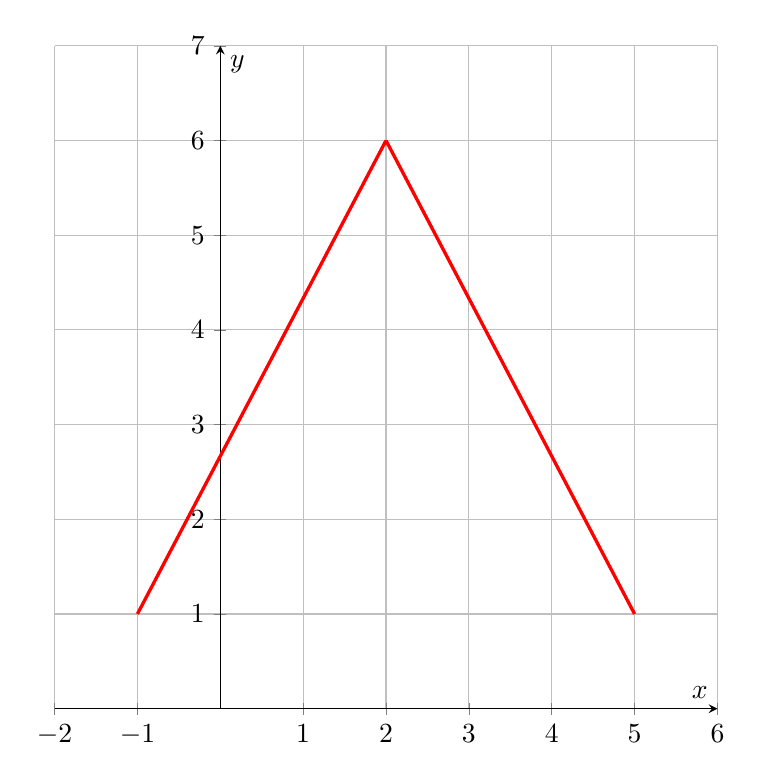
\begin{tikzpicture}
\begin{axis}[
    axis lines=middle,
    width=10cm,
    height=10cm,
    xmin=-2, xmax=6,
    ymin=0, ymax=7,
    xtick={-2,...,6},
    ytick={0,...,7},
    grid=both,
    xlabel=\(x\),
    ylabel=\(y\),
]
% Primer tramo: de x=-1 a x=2
\addplot[domain=-1:2, very thick, red] {5/3*x + 8/3};

% Segundo tramo: de x=2 a x=5
\addplot[domain=2:5, very thick, red] {-5/3*x + 28/3};
\end{axis}
\end{tikzpicture}
\end{center}

\subsection*{Problem 4}
Find the following inverse function.
\[f(x)=\dfrac{5x-7}{-8x+1}\]

\subsection*{Problem 5}
Given the plot of \(y=f(x)\) below, graph the plot of \(y=f^{-1}(x)\).
    \begin{center}
    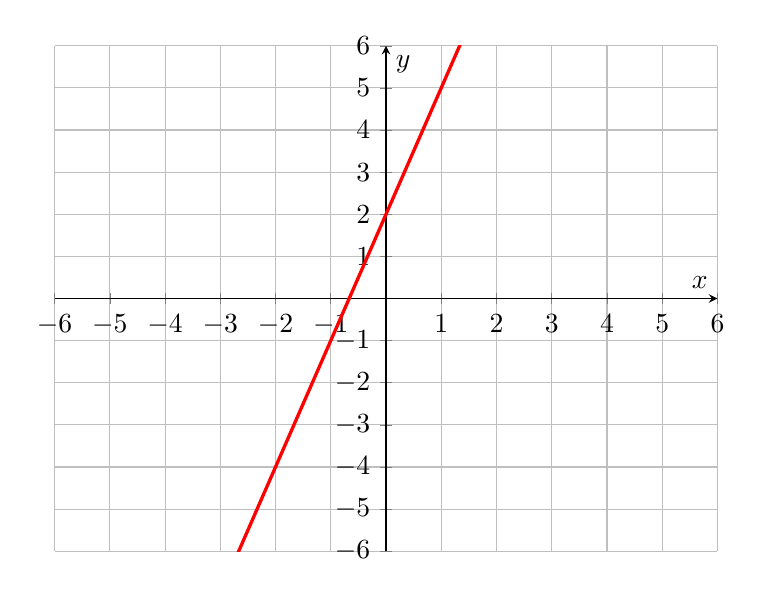
\begin{tikzpicture}
    \begin{axis}[
        axis lines=middle,
        width=10cm,
        height=8cm,
        xmin=-6, xmax=6,
        ymin=-6, ymax=6,
        xtick={-6,-5,...,6}, % Marcas personalizadas en el eje x (de -6 a 6, paso 1)
        ytick={-6,-5,...,6}, % Marcas personalizadas en el eje y (de -6 a 6, paso 1)
        minor tick num=0,    % Elimina marcas menores (opcional)
        grid=both,           % Añade cuadrícula (opcional)
        xlabel=\(x\),
        ylabel=\(y\),
    ]
    \addplot[red, very thick, domain=-4:6, samples=100] {3*x + 2};
    \end{axis}
    \end{tikzpicture}
    \end{center}

\subsection*{Problem 6}
Find the inverse function of \(f(x)=-10x+7\).

\subsection*{Problem 7}
Find the inverse function of \(f\).
\[f(x)=\dfrac{x}{x+2}\]

\subsection*{Problem 8}
Find the inverse function of \(f\).
\[f(x)=\dfrac{2x+3}{5x+4}\]

\subsection*{Problem 9}
Can a function be its own inverse? Explain.

\section*{Problem Set 2\\Difficulty level: Hard}
\subsection*{Problem 1}
For the following exercises, find the inverse function. Then, graph the function and its inverse.
\begin{enumerate}
    \item[(a)] \(\dfrac{3}{x-2}\)
    \item[(b)] \(x^3-1\)
\end{enumerate}

\subsection*{Problem 2}
To convert from \(x\) degrees Celsius to \(y\) degrees Fahrenheit, we use the formula \(f(x)=95x+32\). Find the inverse function, if it exists, and explain its meaning.

\newpage
\section*{Solutions to the Set 1}
\subsection*{Problem 1}
\begin{enumerate}
    \item[(d)] \( f^{-1}(2) = 3 \)
    \item[(e)] \( f^{-1}(8) = -4 \)
\end{enumerate}
\subsection*{Problem 2}
\(g^{-1}(-3)=-1\)
\subsection*{Problem 3}
\([-1,2]\) or \([2,5]\)
\subsection*{Problem 4}
\(f^{-1}(x)=\dfrac{x+7}{8x+5}\)
\subsection*{Problem 5}
The graph should have the points \((2,0),(5,1)(-1,-1)\), etc.
\subsection*{Problem 6}
\(f^{-1}(x)=\dfrac{7-x}{10}\)
\subsection*{Problem 7}
\(f^{-1}(x)=-\dfrac{2x}{x-1}\)
\subsection*{Problem 8}
\(f^{-1}(x)=\dfrac{3-4x}{5x-2}\)
\subsection*{Problem 9}
Yes. The simplest example is \(f(x)=x\), because if we apply the function twice, it returns the original input, such as \(f(f(x))=x\).

\section*{Solutions to the Set 2}
\subsection*{Problem 1}
Check Desmos, GeoGebra or any other graphing calculator to see the graphs of the following inverse functions.
\begin{enumerate}
    \item[(a)] \(\dfrac{2x+3}{x}\)
    \item[(b)] \(\sqrt[3]{x+1}\)
\end{enumerate}
\subsection*{Problem 2}
Assume \(F=y=f(x)\) and \(C=x\). Then, if the original function is \(F=\dfrac{9}{5}C+32\), then the inverse is \(C=\dfrac{5}{9}(F-32)\).
\end{document}
